\documentclass[unknownkeysallowed, 10pt, a4 paper, handout]{beamer}

% Custom beamer theme
\usepackage{../style/beamerthemeCustom}
\newcommand{\HRule}{\rule{\linewidth}{0.5mm}}   %FOR TITLEPAGE

\usepackage{changepage}       % adjustwidth
\usepackage{upquote}
\usepackage{color}
\usepackage{url}
\usepackage{fancyvrb}

\setlength\parskip{0.3cm}

\definecolor{darkgreen}{RGB}{0,100,0}
\newcommand{\green}[1]{\textbf{\textcolor{darkgreen}{#1}}}
\newcommand{\red}[1]{\textbf{\textcolor{red}{#1}}}

\newcommand{\focus}[1]{\textbf{\textcolor{red}{#1}}}
\newcommand{\expire}[1]{\textbf{\textcolor{green}{#1}}}
\newcommand{\ra}{$\longrightarrow$ }
\newcommand{\lra}{$\longleftrightarrow$ }

\newcommand{\code}[1]{\colorbox{black}{\color{green}\texttt{#1}}}
\newcommand{\codeine}[1]{\colorbox{black}{\color{green}\BUseVerbatim{#1}}}

% Command to create two side-by-side minipages
\newcommand{\sidebyside}[5]{
  \begin{minipage}{#1\textwidth}
    #2
  \end{minipage} #3 \begin{minipage}{#4\textwidth}
    #5
  \end{minipage}
}

\title[Linux Programming]{ICTP DP Linux Basic Course - Fortran}
\subtitle{ESP Students - First Semester}
\author[Graziano Giuliani]{Graziano Giuliani \\ \focus{ggiulian@ictp.it}}
\institute[ICTP]{The Abdus Salam International Centre for Theoretical Physics}
\date[\today]{ICTP Diploma Program \\ \today}

\begin{document}


\begin{frame}
  \titlepage
\end{frame}


\begin{frame}[label=outline]
  \frametitle{Course Outline \footnotemark}
  \framesubtitle{Daily program}
  \begin{itemize}
    \item \expire{UNIX/Linux}
    \item \expire{Programming on Linux}
    \item \expire{Text file manipulation}
    \item \expire{Basic BASH and Python}
    \item \focus{Basic Fortran}
      \begin{enumerate}
        \item Program
	\item Modules and Build System
	\item Libraries
      \end{enumerate}
  \end{itemize}

  \vspace{6mm}

  Slides: \\ \code{http://tinyurl.com/2jsvfbd6}
  \vspace{4mm} \\
  or the \LaTeX \ source on GitHub: \\
  \code{https://github.com/graziano-giuliani/LinuxBasics}

  \footnotetext[1]{Course created in 2019 with Adriano Angelone, now LPTMC-FR}
\end{frame}


\begin{frame}[fragile=singleslide]
  \frametitle{Fortran Program}
  \framesubtitle{Text I/O}

  \begin{exampleblock}{Simple I/O Program}
    \begin{verbatim}
program simple_io
  !
  ! This program reads in and prints out a name
  !
  implicit none
  character (len=20) :: first_name

  print *, ' type in your first name.'
  print *, ' up to 20 characters'
  read *, first_name
  print *, ' you enter this name: ', first_name
end program
    \end{verbatim}
  \end{exampleblock}
\end{frame}


\begin{frame}[fragile=singleslide]
  \frametitle{Programming Tips}
  \framesubtitle{Guidelines}

  \begin{enumerate}
    \item Use comments to clarify what is the purpose of program units
    \item Use meaningful variable names
    \item INDENTATION is not mandatory, BUT... DO INDENT!!
    \item Old FORTRAN did allow for implicit definitions: don't use it.
    \item Decide on your own personal conventions and STICK to them
    \item Use appropriate types for variables
    \item Use as much parallelism as possible from the start
  \end{enumerate}
\end{frame}


\begin{frame}[fragile=singleslide]
  \frametitle{Formula Translator}
  \framesubtitle{Why Fortran}

  \begin{enumerate}
    \item Fortran Intrinsic
      \begin{itemize}
        \item \small{\url{https://gcc.gnu.org/onlinedocs/gfortran/Intrinsic-Procedures.html}}
      \end{itemize}
    \item Arrays
      \begin{itemize}
        \item Custom bounds
        \item Slicing and striding
        \item Dynamic allocation
      \end{itemize}
    \item Array operations element by element using implicit loops
    \item Vectorized scalar function using \emph{elemental} keyword
    \item Object orientation and procedure overloading
  \end{enumerate}
\end{frame}


\begin{frame}[label=Fortran, fragile=singleslide]
  \frametitle{Fortran Language}
  \framesubtitle{Programming like in the 1950}
  \begin{columns}[T]
    \begin{column}{.23\textwidth}
      \vspace{30pt}
      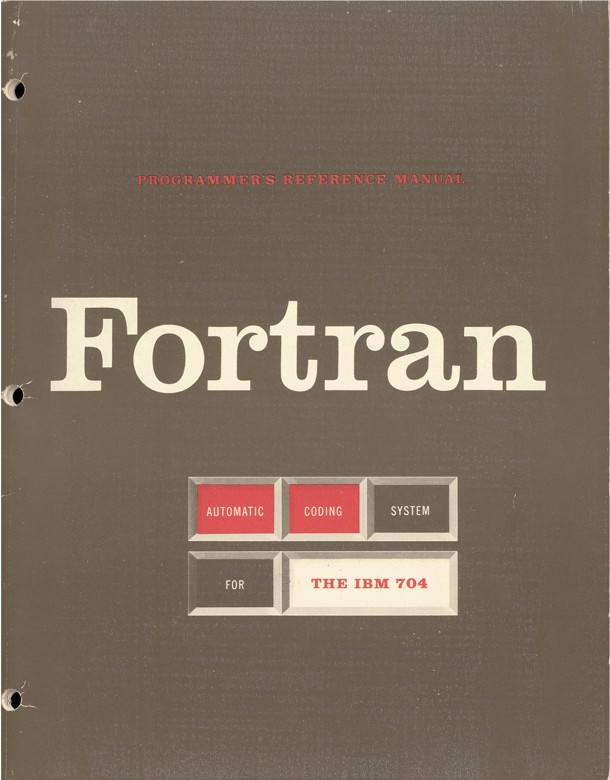
\includegraphics[scale=0.15]{pics/Fortran_acs_cover.jpeg}
    \end{column}
    \hfill
    \begin{column}{.76\textwidth}
      \begin{itemize}
        \item Fortran programs are witten as source text files: \\
          \footnotesize{
            \begin{verbatim}
program count
  integer :: i
  do i = 1, 10
    print *, i
  end do
end program count
            \end{verbatim}
          }
        \item \normalsize{A \focus{compiler program} parses source files and
            create binary object files:} \\
          \footnotesize{
          \code{gfortran -o myprog myprog.f90}
          }
        \item \normalsize{Objects are linked with other objects or
           libraries to create executables:} \\
          \footnotesize{
            \begin{verbatim}
0000000 457f 464c 0102 0001 0000 0000 0000 0000
0000010 0003 003e 0001 0000 06f0 0000 0000 0000
0000020 0040 0000 0000 0000 1a78 0000 0000 0000
0000030 0000 0000 0040 0038 0009 0040 001d 001c
0000040 0006 0000 0004 0000 0040 0000 0000 0000
            \end{verbatim}
          }
      \end{itemize}
    \end{column}
  \end{columns}
\end{frame}


\begin{frame}[label=exercise1, fragile=singleslide]
  \frametitle{Exercise}
  \framesubtitle{Write and compile Fortran 'Hello World'}
  \begin{itemize}
    \item Create a text file \code{hello.f90} with the below content:
      \footnotesize{
      \begin{verbatim}
program hello
  implicit none
  integer , parameter :: stdout = 6
  character(len=*), parameter :: message = 'Helo World'
  character(len=1), parameter :: mark = '!'
  write(stdout,'(a,a)') message, mark
end program hello
      \end{verbatim}
      }
    \item Compile the program into an executable file: \\
      \code{gfortran -o hello hello.f90}
    \item Execute the executable file created: \\
      \code{./hello}
  \end{itemize}
    \begin{alertblock}{Have you noticed?}
      No error is allowed in the code: Fortran Language has very
        strict syntax. But you can misspell the message! \\
      Why we had to run the program with \code{./hello}?
    \end{alertblock}
\end{frame}


\begin{frame}[label=compiler]
  \frametitle{Compiler flags}
  \framesubtitle{Optional arguments for Fortran programming}
  The compiler is a program and accepts command line arguments. Above we
    have used the \code{-o} option to specify the name of the output.
  \begin{block}{Useful gfortran options}
    \begin{itemize}
        \item \code{-o program} output program name (default a.out)
      \item \code{-Ofast} Optimize program for fast execution time
      \item \code{-O0} Remove all optimization (for debugging)
      \item \code{-g} include debugging information
      \item \code{-Wall} Enables commonly used warning options pertaining to
          usage recommend avoiding and that are easy to avoid
      \item \code{-pedantic} check program for Fortran standard conformance
      \item \code{-fcheck=all} perform all available run-time checks
      \item \code{-fbacktrace} print the whole trace of the error
  \end{itemize}
  \end{block}
\end{frame}


\begin{frame}[label=exercise2, fragile=singleslide]
  \frametitle{Exercise}
  \framesubtitle{Debug a Fortran program}
  \begin{itemize}
    \item Create a text file \code{error.f90} with the below content:
      \footnotesize{
\begin{verbatim}
program error
  implicit none
  integer, parameter :: im = 2
  integer, dimension(im,im) :: matrix
  integer :: j
  do j = 1 , 2*im
    do i = 1 , 2*im
      matrix(i,j) = i*j
      print*, matrix(i,j)
    end do
  end do
end program error
\end{verbatim}
      }
    \item Compile and correct the error
    \item Run the program and check the runtime error
    \item Compile in debug:
        \code{-O0 -g -Wall -pedantic -fcheck=all -fbacktrace}
    \item Run the program, check the error and correct the program
    \item Recompile an optimized executable
  \end{itemize}
\end{frame}

\begin{frame}[label=exercise_num, fragile=singleslide]
  \frametitle{Program Example}
  \framesubtitle{A numerical Exercise}
  \begin{itemize}
    \item Assignment from Numerical
      \footnotesize
{
\begin{verbatim}
 Write a program that solves the differential equation
    dx/dt = -x using
 1) Euler method
 2) midpoint methods.
 Create separate subroutines for the two methods.
 Solve with initial conditions x(0.0) = 1.0 and dt=0.1,
 N=100 and store the results in arrays tlist and xlist.
 The program should create a file for each method with
 the result in two columns: t and x(t).
 Plot the result x versus t with your favorite plotting
 program.
 Submit the graphs and your code.
\end{verbatim}
}
  \end{itemize}
\end{frame}

\end{document}
